\chapter{{Introduction}}
\label{ch_1:intro}
\begin{figure}
	\centering
	\begin{minipage}{1.1\textwidth}
		\centering
		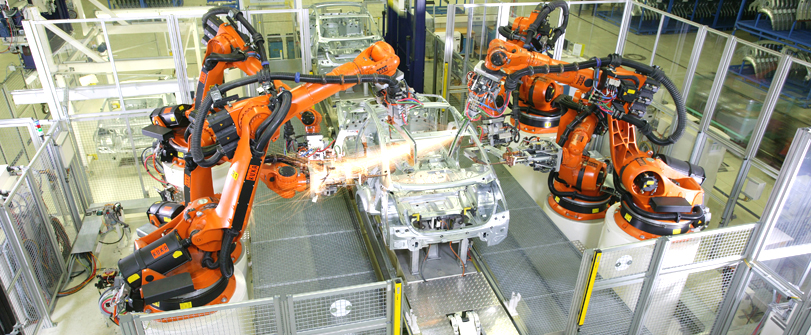
\includegraphics[height=5cm,keepaspectratio]{Chapter1/fig/factory}
		\captionof{figure}{Robotics in Factory (Source: Kuka Robot)}
		\label{fig:RF}
	\end{minipage}
	\begin{minipage}{.5\textwidth}
		\centering
		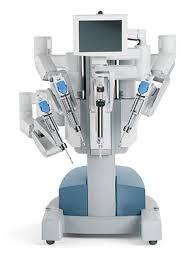
\includegraphics[height=5cm,keepaspectratio]{Chapter1/fig/healthc}
		\captionof{figure}{Health Care\\ (Source:  da Vinci Surgical System)}
		\label{fig:HC}
	\end{minipage}%
	\begin{minipage}{.5\textwidth}
		\centering
		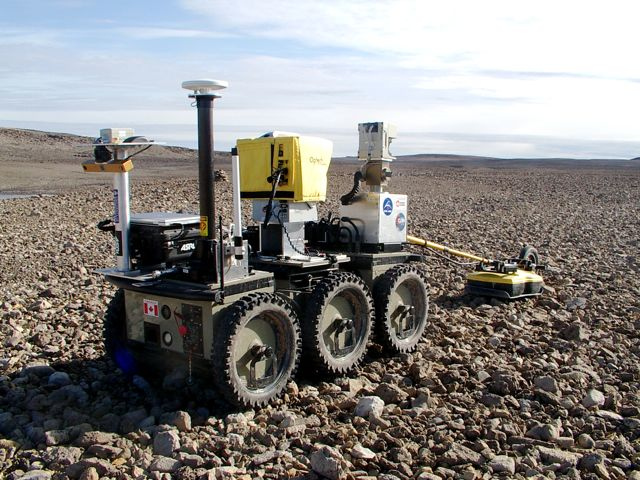
\includegraphics[width=.8\linewidth,height=5cm,keepaspectratio]{Chapter1/fig/explore}
		\captionof{figure}{Exploration and surveillance\\ Source: Autonomous Space Robotics Lab - University of Toronto}
		\label{fig:ES}
	\end{minipage}
\end{figure}
The use of robots such as robotic arm shown in Figure \ref{fig:RF} has been used in factories for a long time, basically for repetitive kind  of job. Though it started with the intention to reduce human labour, production cost, and increased productivity, with technological development  their scope has expanded beyond  manufacturing domain. Robots are now being used for health care, surveillance, exploration, etc. as illustrated in Figures \ref{fig:HC} and \ref{fig:ES}. The reduction in development cost  has resulted in introduction of robotic systems in entertainment industries and personal care as well. Robots have matured from heavy duty serial linked mechanical arms to a more presentable form such as ASIMO ( Figure \ref{fig:HAsimo}) by Honda and Aibo by Sony  ( Figure \ref{fig:SA}).  
\begin{figure}
	\centering
	\begin{minipage}{.5\textwidth}
		\centering
		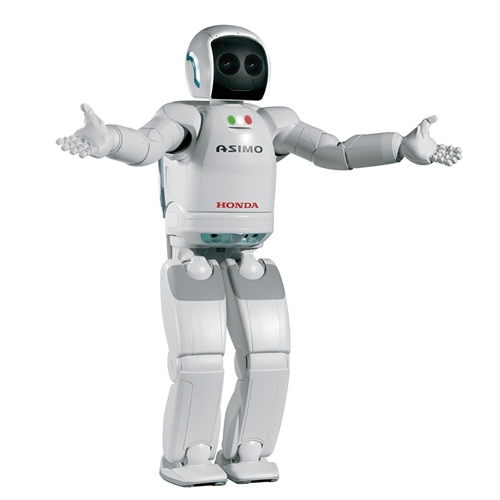
\includegraphics[height=5cm,keepaspectratio]{Chapter1/fig/Honda-Asimo}
		\captionof{figure}{Honda Asimo \\Source:http://asimo.honda.com}
		\label{fig:HAsimo}
	\end{minipage}%
	\begin{minipage}{.5\textwidth}
		\centering
		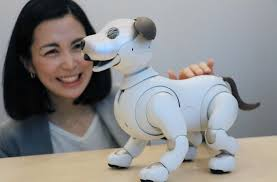
\includegraphics[width=.8\linewidth,height=5cm,keepaspectratio]{Chapter1/fig/aibo}
		\captionof{figure}{Sony Abio\\ Source: https://us.aibo.com/}
		\label{fig:SA}
	\end{minipage}
\end{figure}

 In areas where human access is not preferred or restricted  due to risk of life or inhospitable environmental conditions as in chemical, space or nuclear industries, robotic systems have gained huge popularity in providing services as surveillance, rescue, exploration and remote maintenance.  Research in teleoperated and autonomous mobile robotics has been fuelled largely by these  requirement. Teleoperated mobile robots are suitable for these applications  as the workspace required to be covered is very large, and it is essential to maintain  physical separation between the robot and its control station. Moreover, the remote environment is in general unknown. 
 
 The present research too was motivated by a similar requirement for in-situ measurement of the radioactive radiation, mostly neutron field, inside the vault and cave areas of   K-130,  K-500  and Medical Cyclotron operational at VECC, Kolkata, West Bengal. Cyclotrons are used to accelerate  charged particles to high energies. These are required for experiments in nuclear physics and nuclear medicine. The particles are accelerated to high energy using a high frequency alternating voltage which is applied between two hollow "D"-shaped sheet metal electrodes called "Dees" inside a vacuum chamber. The area surrounding the Dee is called the vault.  The cave is the area where beam line (beam of  accelerated charged particles) is available for experimentation. Radiation mapping of these areas are  mandatory requirements for getting safety clearance from regulators during  commissioning of new units and at regular intervals during operational life of the cyclotron facility.   Though, there are radiation detectors placed at different locations in these areas they can only measure radiation levels at discrete locations, but can not provide the 3-D radiation  map. The advantage of having a  radiation map is that it  provide detailed  input to health physicist  of the dose a person may receive and accordingly plan emergency  operations. These maps also provide the plant operators with the location of radiation leakage and accordingly tune the system to improve its efficiency.

The challenge faced for in-situ inspection during operation of cyclotron is that the interaction  between  an  accelerated  beam   of  charged  particles  and  the  target  produce Bremsstraghlung and characteristic x-rays, prompt $\gamma$-rays, neutrons and delayed radiation ($\beta $ and $\gamma$) this makes human presence unacceptable.  A teleoperated mobile robot with wireless communication link is the obvious solution. This thesis discusses the design, analysis and development of a prototype robot  to carry out in-situ measurement and mapping of radiation level.

\section{Research Contributions}
The original contributions of the present research are listed below:
\begin{enumerate}[(i)]

\item Design of a customized teleoperated mobile robot for remote surveillance and mapping application.
\item Development of kinematic and dynamic models of the robot at hand.
\item Control architecture required for intuitive teleoperation of this mobile robot.
\item Predictive visual feedback  to alleviate problem arising due to time delay.


\end{enumerate}
\section{Thesis Organization}
The thesis contains eight chapters and three appendix. They are organized as follows:
\paragraph*{Chapter 1: Introduction\\}
This  chapter, discusses the scope of mobile robotics in general and the motivation which led to this research work.
\paragraph*{Chapter 2: Literature Review\\}
This chapter presents the literature review in the following areas: \textit{kinamatics and dynamics} of mobile robots, \textit{control of mobile robot}, \textit{control for time delay systems}, \textit{performance of operator under tele-operation},  and \textit{predictive display systems}.

\paragraph*{Chapter 3: Design of a Mobile Robot\\}
This chapter highlights the design considerations of a tele-operated mobile robot based on mission requirements and  environmental conditions.  It  discusses the mechanical design for the traction system, the steering gear, and the scissor mechanism. Selection of  steering system based on terrain condition and power requirement is also discussed.   
\paragraph*{Chapter 4: Dynamics of Wheeled Mobile Robots \\}
In this chapter, the dynamic equations of a four wheeled differentially driven robotic platform derived using natural orthogonal compliment method is presented. The platform has two actuated wheels and two passive wheels. Different types of passive wheels were studied and  corresponding dynamic equations were derived. 
\paragraph*{Chapter 5: Control of a mobile manipulator \\}
The control architecture and the hardware used for tele-operation is presented along with the detailed description of implementation of the controller software at both the remote (mobile robot)  and the local station. The experimental results of robots position based on wheel odometry and is torque requirement for few predefined paths are presented. 

\paragraph*{Chapter 6: Simulation of Tele-operation \\}
In this chapter simulation of a teleoperated mobile robot is presented both without time delay and  under time delay due to communication link. It is shown via simulations that with increase in time delay,  teleoperation loop become unstable. 
 
\paragraph*{Chapter 7: Predictive Display \\}
In this chapter,  we propose a Predictive Display strategy to counter the time delay in video feedback by extrapolating in time  the camera view based on the predicted position of the robot at remote location. 

\paragraph*{Chapter 8: Conclusions\\}
This chapter summarizes major results of this research work. Limitations of the system along with the future scope of work based on present experiences are also addressed.


\paragraph*{Bibliography}
\paragraph*{Appendix A:  Measurement of Time Delay in Video Feedback  \\}
Here the experimental set up and methodology used to determine the time delay is presented.
\paragraph*{Appendix B:  Stability of Pure Pursuit  under Time Delay \\}
Based on the paper by Ollero \cite{ollero1995stability} stability analysis of pure pursuit tracking algorithm with input delay is discussed.
\paragraph*{Appendix C:  Optimal Design of Steering Linkages \\} 
This appendix describes the formulation of optimization problem for steering linkage.